\section{Models for Density (Median)}

We fit a variety of competing linear models using the `lm' function in R \citep{Rprogram}. We used the median transformed CT of the technical replicates as our response variable. Initially, we fit a simple linear model, l.one.line, where we fit a least squares line of best fit for our response variable by considering only a single input predictor, log2(Biomass). To plot models, we used the base R plot function and the ggplot2 package \citep{ggplot}, as well as the `ggthemes' package \citep{ggthemes} and the `latex2exp' package\citep{latextoexp}. Next, we fit two multiple linear models. The first model named lmparallel.tfac is a multiple linear model with the two predictors, Log2(Biomass) and tank. We also fit a model called lfull.tfac, which incorporates both Log2(Biomass) and tank and also the interaction between Log2(Biomass) and tank.


\begin{figure}[H]
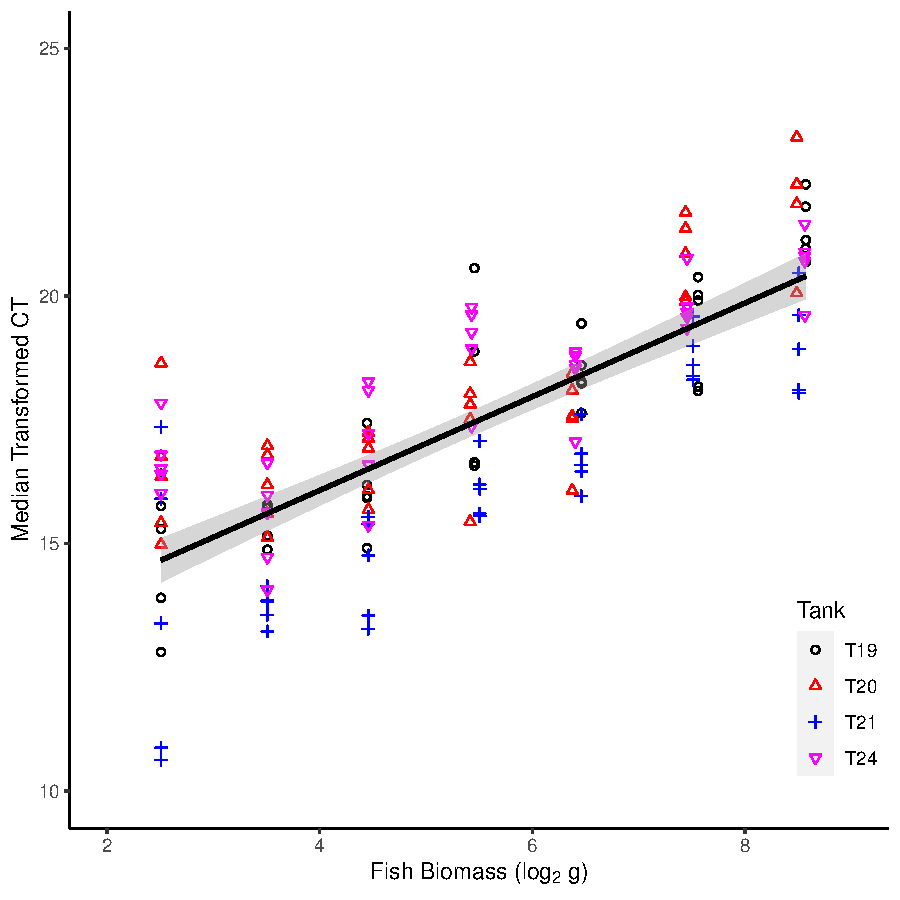
\includegraphics{Chapter3Images/ggplotnew.pdf}
\caption{ Median Transformed CT versus Log2(Biomass). The fitted regression line, l.one.line and the 95 \% confidence intervals are included. Each of the four tanks has an associated color and shape.}
\label{fig:medct1}
\end{figure}

%\begin{table}[H]
 %\begin{singlespace*}
%\verbatiminput{tablesandimages/loneline.txt}
%\caption{Summary of our first simple model,  l.one.line. This model only includes an intercept and a biomass term.}
%\label{lab:loneline}
%\end{singlespace*}
%\end{table}


\begin{table}[H]
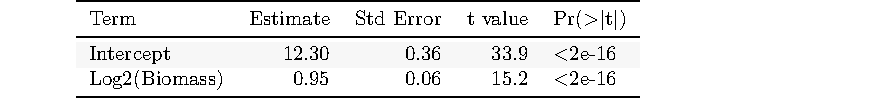
\includegraphics{Chapter3Images/lonelinekable.pdf}
\caption{Summary of our first simple linear model,  l.one.line. This model only includes an intercept and a biomass term. The $R^{2}$ value is 0.626.}
\label{lab:loneline}
\end{table}


Table~\ref{lab:loneline} is a summary of a simple linear model (l.one.line)  fit using the lm function. The estimated intercept of the model is 12.30 with a standard error of 0.36. The model also produces an estimate for the slope of 0.95 with a standard error of 0.06.  The p-value for both estimates is very small. The p-values are in the $Pr(>|t|)$ column. The p-value refers to the probability that we observe what we did, given that the null hypothesis is true. The null hypothesis in this case is that the associated parameter is zero. Since the p-value is so small, we can reject the null hypothesis (at a significance level of 0.05) and conclude that those terms are significantly different from zero. 

\vspace{12pt}


Figure~\ref{fig:medct1} confirms visually that as fish biomass increases, Log2(Biomass) in particular, median TCT also increases. This makes sense, as with more fish we would expect more residual eDNA, and thus a lower CT score (and hence a higher TCT score). The $R^{2}$ is $0.626$ which means that this simple model already does a relatively good job at explaining variation in the data.

\newpage

We also plot regression lines obtained by considering each tank on its own and allowing the intercept to vary. 


\begin{figure}[H]
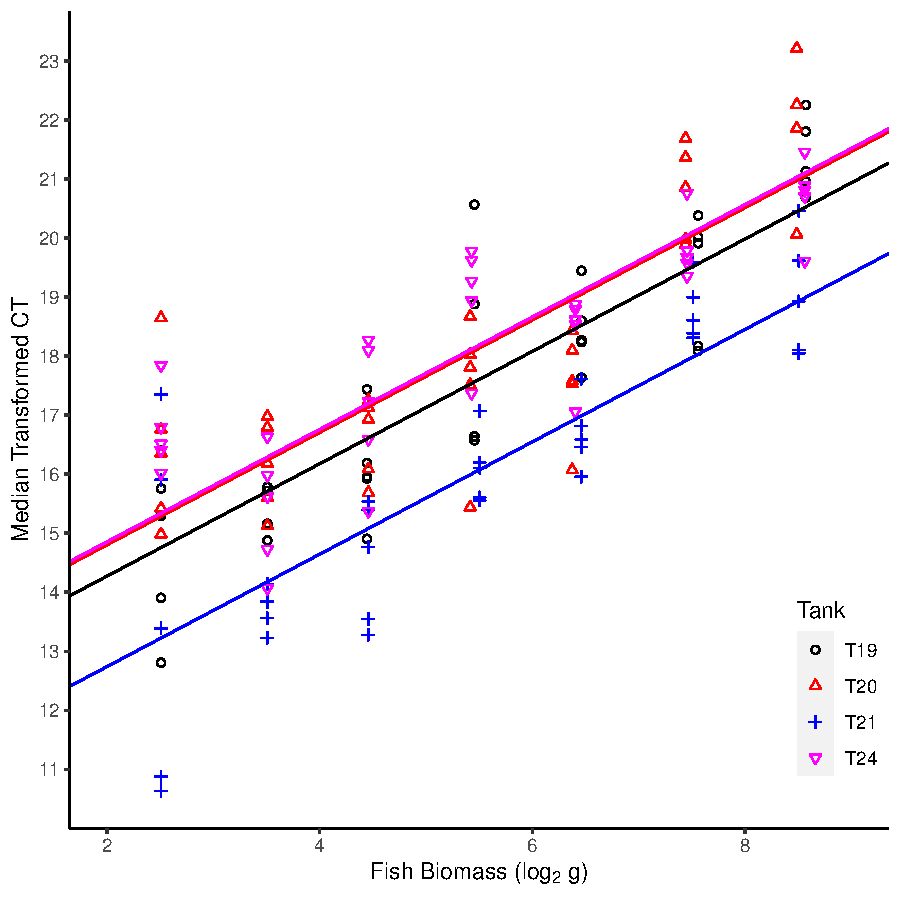
\includegraphics{tablesandimages/parfits.pdf}
\caption{ Lines of best fit for Median Transformed CT versus Log2(Biomass) for each specific tank. This is equivelent to the model  lmparallel.tfac.}
\label{fig:medpar}
\end{figure}

Figure~\ref{fig:medpar} is the plot of the model  lmparallel.tfac. In this model, only the intercept is allowed to vary for each tank, but the slope remains the same. We see again tank 21 has a siginficantly lower intercept than the other tanks.


\vspace{5mm}

% \begin{table}[H]
 %\begin{singlespace*}
%\verbatiminput{tablesandimages/lmparallel.txt}
%\caption{This model, lm.tfac considers each tank as a predictor.}
%\label{lab:lmparallel}
%\end{singlespace*}
%\end{table}

 \begin{table}[H]
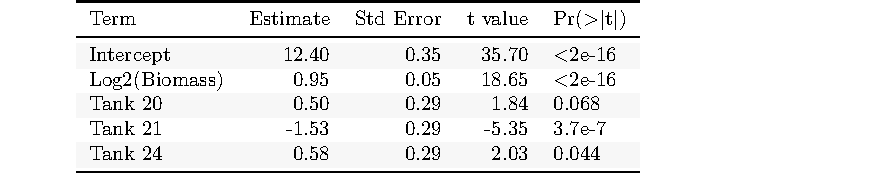
\includegraphics{Chapter3Images/lmparallelkable.pdf}
\caption{Parameter estimates and standard errors for model  lmparallel.tfac where Log2(Biomass) and tank are predictors. The $R^{2}$ value is 0.756.}
\label{lab:lmparallel}
\end{table}



Table~\ref{lab:lmparallel} provides a summary for the model  lmparallel.tfac. This model has a common slope parameter for Log2(Biomass), but allows the intercept to change for each tank.  The intercept changes depending on which tank the point belongs to according to the estimates in Table~\ref{lab:lmparallel}.The baseline for tank comparisons is tank 19. Compared to tank 19, tank 20 and tank 24 appear to result in slightly higher median TCT values. This can be seen by the coefficients that are greater than 0, which means for those tanks we have in increase in median TCT compared to our baseline tank. For tank 24, the p-value is $0.044$, which indicates significance. However, we see a clear effect in Tank 21, which results in a lower median TCT compared to the other tanks, with a very small p-value of 3.7e-07 indicating strong evidence at the 0.05 alpha level. One possible explanation for this is that tank 21 obtained a more complete bleaching than the other tanks, hence resulting in less eDNA when sampled. This would cause a higher CT and hence a lower TCT.  The adjusted $R^{2}$ for this model is $0.746$, which is much larger than the adjusted $R^{2}$ of l.one.line (0.623). This means that our model does a good job at explaining the variation in the data. The adjusted $R^{2}$ contains a penalty term for the number of predictors in the model. 





\newpage

Finally, we also consider a model that includes the possible interactions between tank number and biomass.  This model allows for a different slope and intercept for each tank and also allows for interactions between tank and biomass. This is the model plotted in Figure~\ref{fig:lmedspecific}, and we will see that results obtained from this model are equivelent to considering each tank in isolation.

\begin{figure}[H]
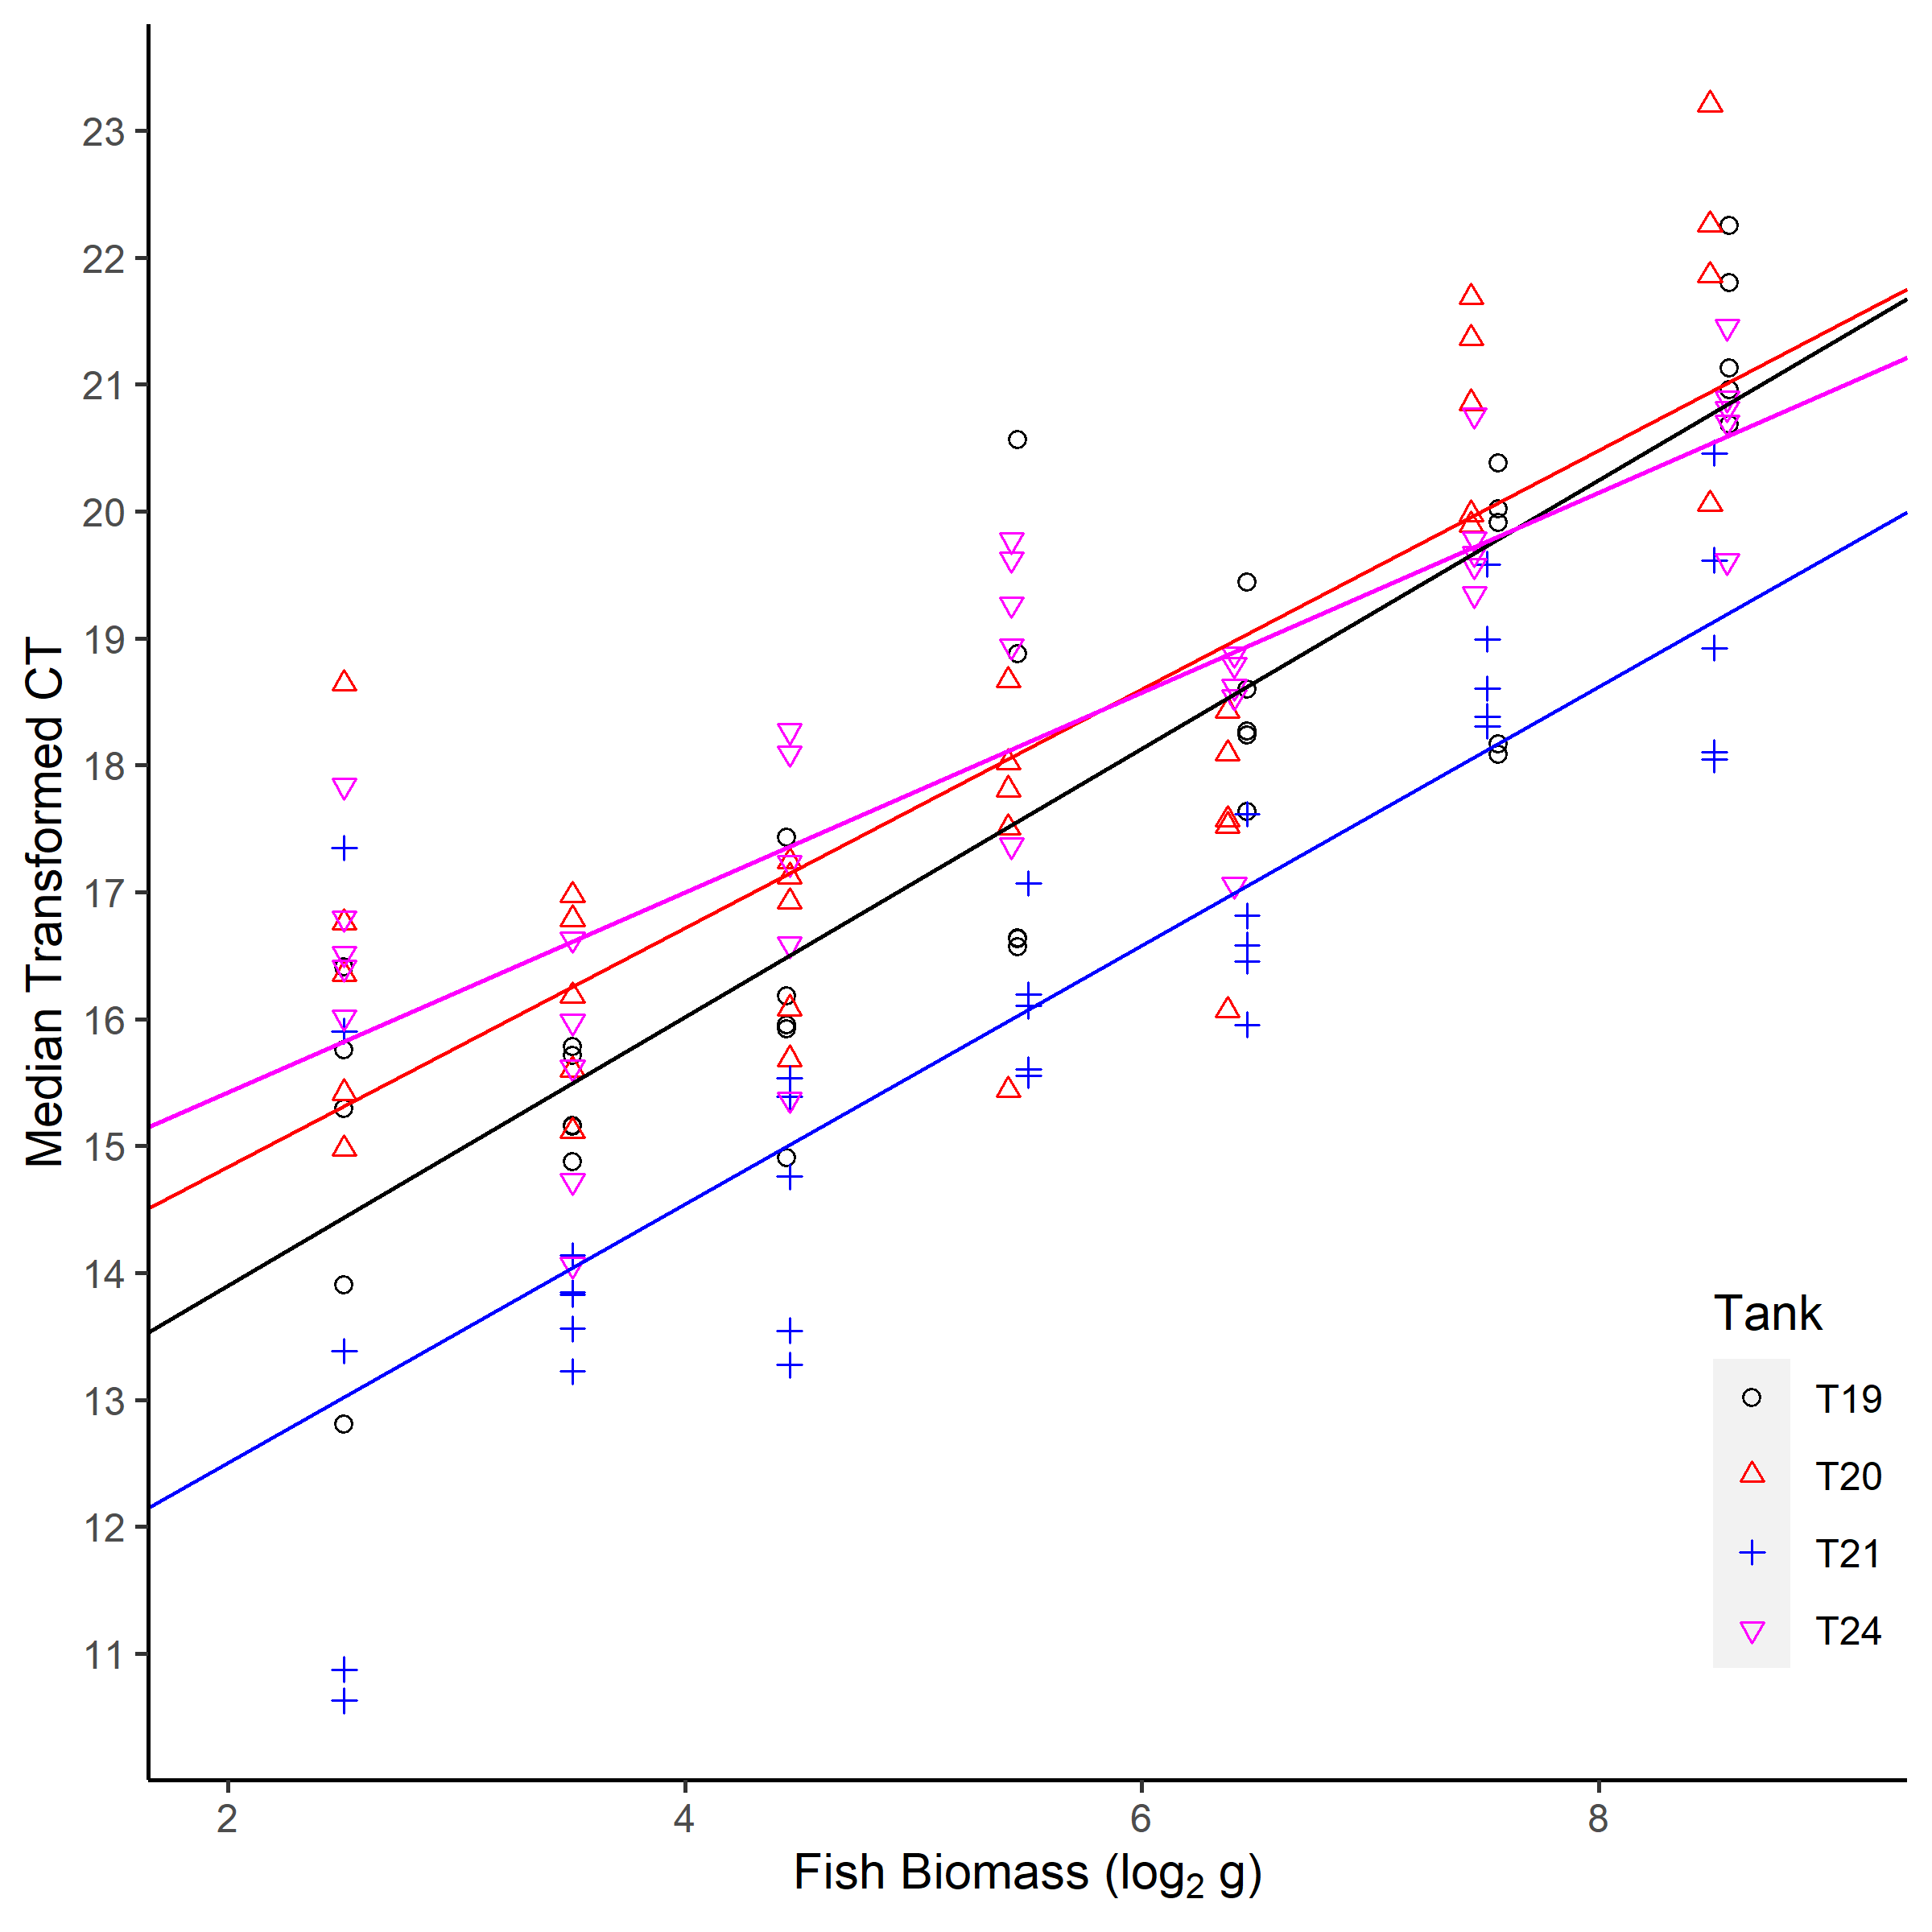
\includegraphics{Chapter3Images/ggplotnew2.png}
\caption{ Lines of best fit for Median Transformed CT versus Log2(Biomass) for each specific tank. This is equivelent to the model lfull.tfac.}
\label{fig:medct33}
\end{figure}

Figure~\ref{fig:medct33} is a plot of regression lines obtained by applying regression over each individual tank. In this regression, each tank has its own intercept and own slope. Figure~\ref{fig:medct33} seems to indicate that tank likely impacts the result of median TCT. Thus we fit a model that included tank as a predictor. 



\begin{table}[H]
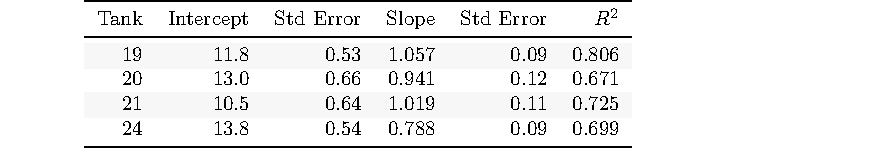
\includegraphics{tablesandimages/sumtable1.pdf}
\caption{Table summarizing simple linear regression on Log2(Biomass) when each tank is considered in isolation for median TCT.}
\label{fig:lmedspecific}
\end{table}



Table~\ref{fig:lmedspecific} summarizes the results of applying simple linear regression to each tank in isolation, obtaining separate estimates for each intercept and slope. Tank 21 has the smallest intercept, while tank 24 has the largest intercept. The slopes are similar, however tank 24 has a noticeably smaller slope. The $R^{2}$ are all quite high, but tank 19 alone has the highest $R^{2}$. 



   \vspace{12pt}



\begin{table}[H]
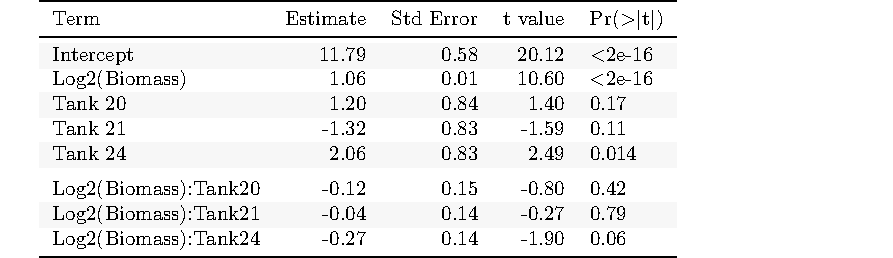
\includegraphics{Chapter3Images/lfulltfac.pdf}
\caption{Parameter estimates and standard errors for the model model, lfull.tfac. This model allowed for interactions between all terms. The $R^{2}$ value is 0.763.}
\label{fig:lfulltfac2}
\end{table}

Table~\ref{fig:lfulltfac2} provides a summary for the full model (lfull.tfac) that includes interactions. We obtain similar estimates to Table~\ref{lab:lmparallel}. However, we now have included interactions. The interaction terms are not statistically significant.  Thus, the interaction between tank and biomass in our modelling is not warranted. This is further evidence that accounting for biomass as a predictor in insolation may be warranted. Notice we obtain identical parameter estimates to those given in Table~\ref{fig:lmedspecific}.

\newpage

We apply ANOVA to compare the current models:

   \vspace{12pt}



\begin{table}[H]
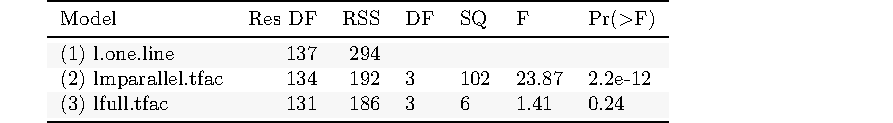
\includegraphics{tablesandimages/anova1.pdf}
\caption{Summary of the additional sum of squares test comparing l.one.line,  lmparallel.tfac and lfull.tfac.}
\label{fig:anovacompare2}
\end{table}


Table~\ref{fig:anovacompare2} provides the results of applying ANOVA on the three previously models. We use an additional sum of squares test to compare the models. We are testing the significance of the three models sequentially. Model 3, lfull.tfac allows for both the slopes and intercepts to change and it also allows for interactions between the terms. Model 2, lfull.tfac, has constant slopes but differing intercepts. Hence the test of model 3 versus model 2 is a test of the hypothesis of a common slope versus different slopes. Since we have a large p-value (0.24), we can conclude that the additional slope parameters are not significantly different from zero. The comparison between model 2 and model 1 is the test of non-differing intercepts for each tank. Because the p-value for this test is so low, we reject this hypothesis. That is, since the p-value (2.2e-12) is so small, we safely reject the null hypothesis (at the 0.05 significance level). Hence, the effect of tank (and hence differing intercepts) is significant and should be included in any modeling. 

\newpage

We now fit a model similar to l.one.line. However, we now collapse over each tank by taking the median value of TCT for each tank. This model is called l.tankregression.med.

   \vspace{12pt}

\begin{figure}[H]
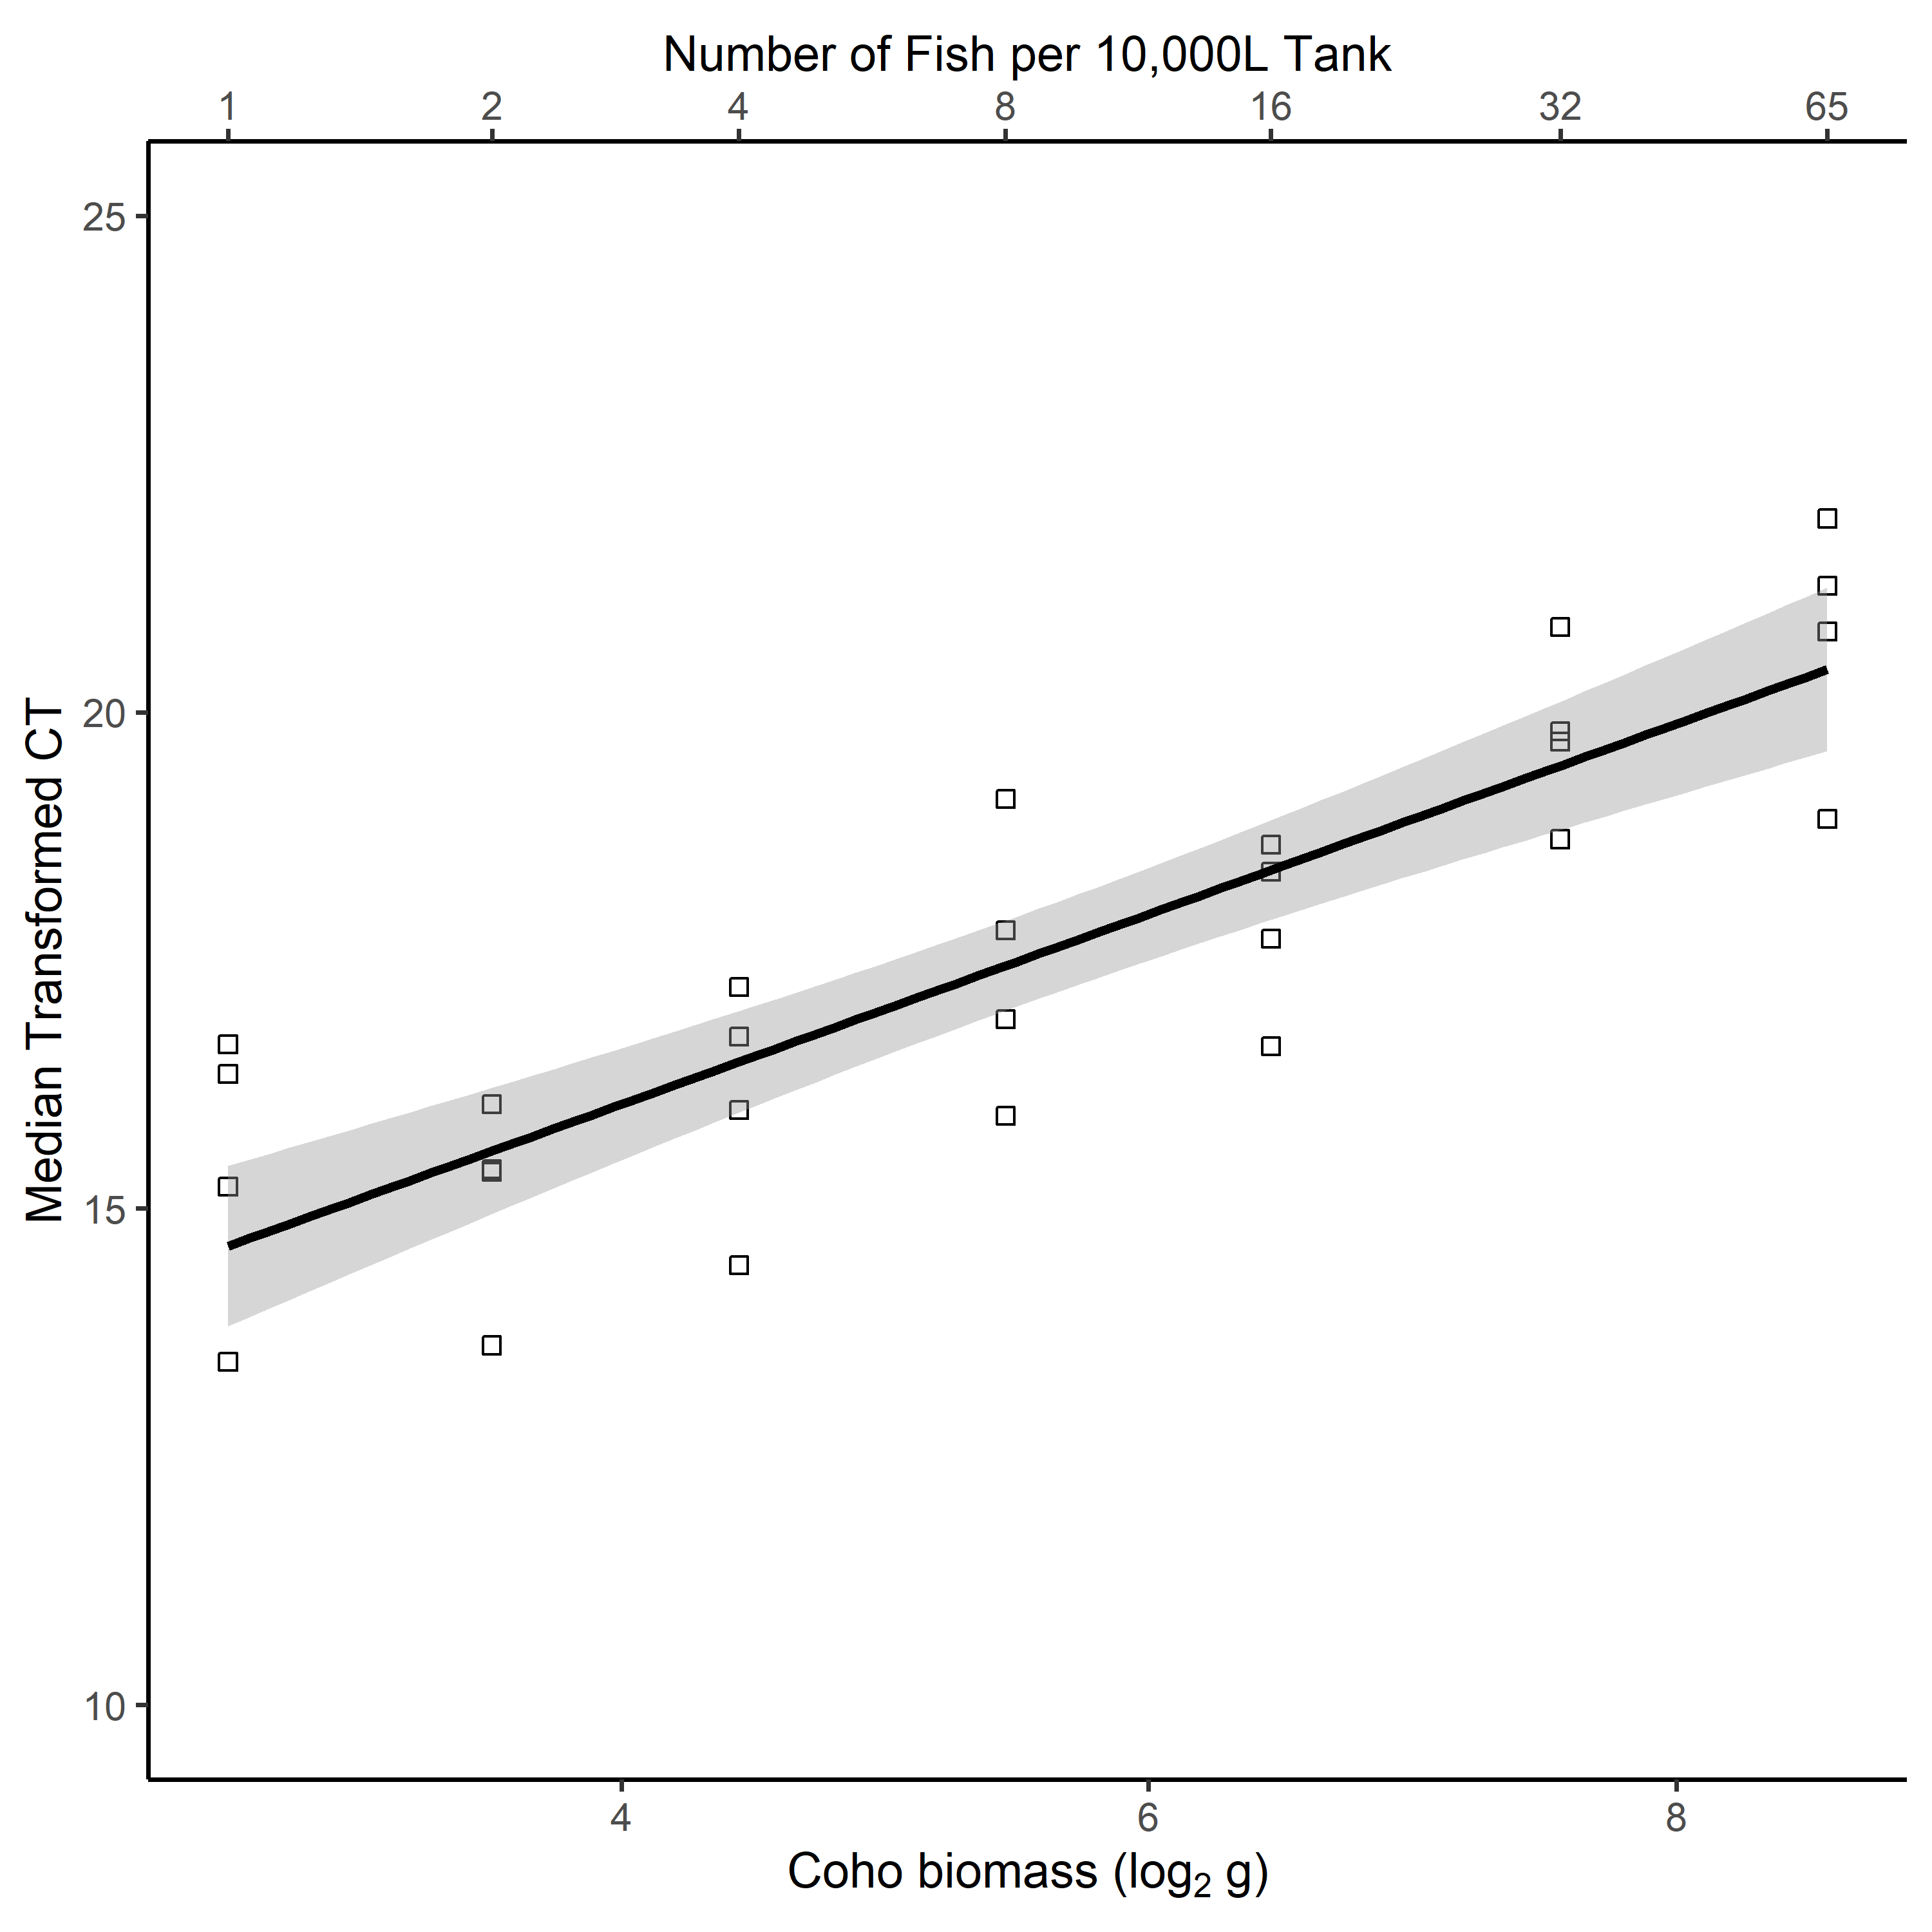
\includegraphics{Chapter3Images/ggplotnew5.png}
\caption{ \hspace{1mm}   Regression line showing the relationship between biomass and Median TCT. Included are the confidence bands about the regression line.  The line is the model l.tankregression.med. The $R^{2}$ is 0.748. Points shown represent the Median TCT for each of the four tanks for each of the seven unique numbers of fish.
}
\label{fig:medct44}
\end{figure}




\begin{table}[H]
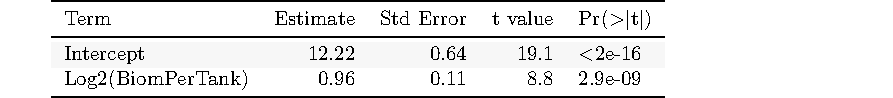
\includegraphics{Chapter3Images/tankregressionMED.pdf}
\caption{Parameter estimates and standard errors for the model l.tankregression.med. This model took the median TCT over each tank for each number of fish. The $R^{2}$ value is 0.748. }
\label{fig:lrankmed}
\end{table}

 Figure~\ref{fig:medct44} is a plot made of our final model, l.tankregression.med. Each point represents the Median TCT for each of the four main tanks. Each distinct biomass value corresponds to a unique number of fish.  The results of this final model are good, as we have quite a large $R^{2}$ value. Table~\ref{fig:lrankmed} summarizes the result of taking the median of TCT over each tank and fitting a simple linear regression model. The only independent variable considered is log2 of Coho biomass. By collapsing over each tank, we were able to capture a large portion of the variation in our data.




